\documentclass[final]{beamer}
\usetheme{RJH}
\usepackage[width=180,height=120,scale=1.5,debug]{beamerposter}
\usepackage[absolute,overlay]{textpos}
\setlength{\TPHorizModule}{1cm}
\setlength{\TPVertModule}{1cm}

\usepackage{graphicx}
\usepackage{caption}
\usepackage{subcaption}

\title{Modular Inverse Reinforcement Learning on Human Motion}
\author{Shun Zhang, Matthew Tong, Mary Hayhoe, Dana Ballard\\
Department of Computer Science, Center of Perceptual Systems\\
University of Texas at Austin}
\footer{}

\begin{document}
\begin{frame}{} 

% left
\begin{textblock}{37}(1,8)
\begin{block}{Introduction}
\begin{itemize}
\item
Humans are able to learn and carry out very complex tasks involving 
many different objectives, while most reinforcement learning algorithms suffer
from the curse of dimensionality.
\item
One promising possibility is that the complex task can be broken down into 
{\bf sub-tasks} that are each learned separately.
\item
This {\bf decomposition} allows the behavior in the complex task to be chosen based on
the value of a weighted sum of individual sub-tasks.
\item
Our experimental analysis shows that the modular reinforcement can be a 
good model of predicting {\bf human subjects'} sub-task priorities in a way that
explains their behavioral choices.
\item
We use the {\bf Modular Inverse Reinforcement Learning} approach to analyze
human subjects' behaviors.
\end{itemize}
\end{block}

\begin{block}{Modular Inverse Reinforcement Learning}
\begin{itemize}
\item {\bf MDP decomposition.}
\item {\bf Modular Reinforcement Learning.}
We assume that the global Q function is a weighted
sum of all $Q_i$, where $Q_i$ is the Q function for i-th module.
$$Q(s, a) = \sum_i w_i Q_i (s_i, a)$$
where $w_i$ is the weight of the i-th sub-MDP. $w_i \geq 0, \sum_i w_i = 1$.
$s_i$ denotes the decomposition of $s$ in the i-th module.
\item {\bf Modular Inverse Reinforcement Learning.}
We maximize the objective function
$$\max_w \prod_t \frac{e^{\eta Q(s^{(t)}, a^{(t)})}}{\sum_b e^{\eta Q(s^{(t)},
b)}}$$
where $s^{(t)}$ is the state at time $t$, and $a^{(t)}$ is the action at time
$t$, which are both from samples. $Q(s, a) = \sum_i w_i Q_i(s_i, a)$, as defined
before. $\eta$ is a hyperparameter that determines the consistency of human's
behavior.
\end{itemize}
\end{block}
\end{textblock}

% middle
\begin{textblock}{37}(40,8)
\begin{block}{Multi-objective Domain}
\begin{figure}[h]
\centering
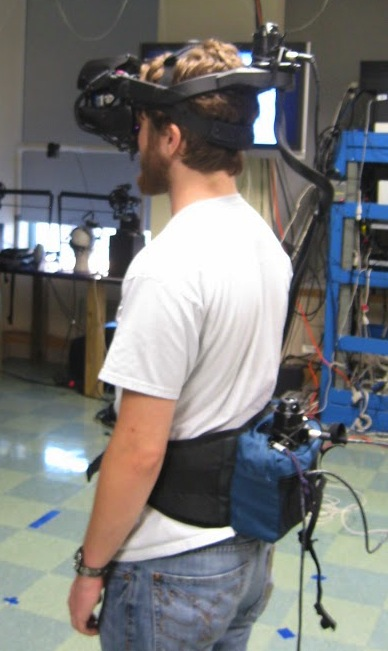
\includegraphics[width=0.2\textwidth]{human.jpg}
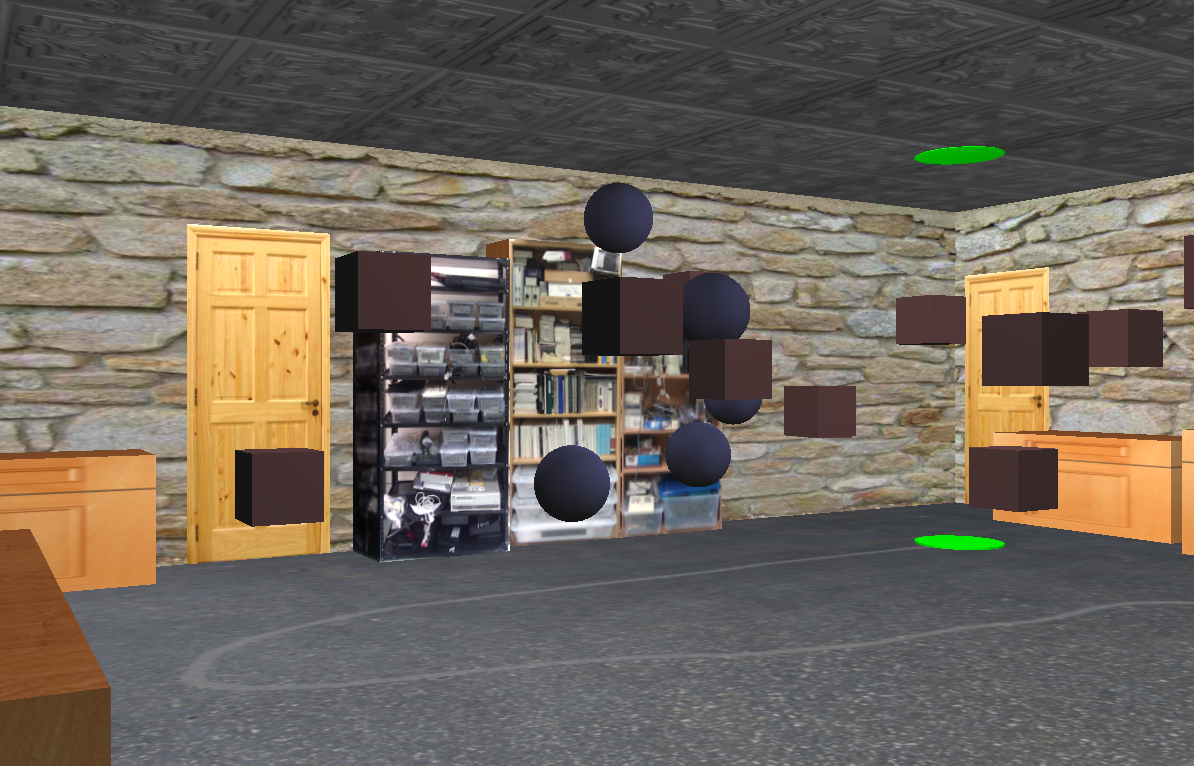
\includegraphics[width=0.6\textwidth]{env.png}
\caption{(Left) A human subject with a head mounted display (HMD) and trackers
for the eye, head, and body.  (Right) The environment the human can see through
the HMD.  The red cubes represent obstacles. The blue balls represent targets.
There is also a gray path on the ground that the human subject can follow.}
\label{fig:avatar}
\end{figure}
\end{block}

\begin{block}{Experiments}
\begin{figure}[h]
\centering
\begin{subfigure}[b]{0.4\textwidth}
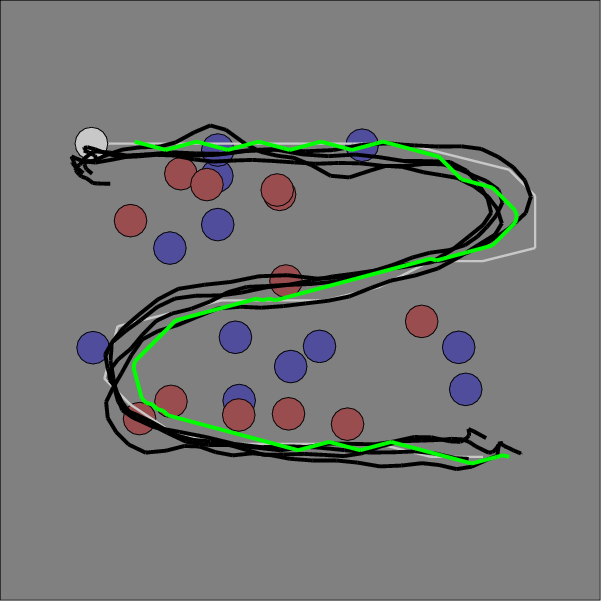
\includegraphics[width=\textwidth]{task_1.png}
\caption{Path module only,\\$w = (0.039, 0.0, 0.960)$. }
\end{subfigure}
\begin{subfigure}[b]{0.4\textwidth}
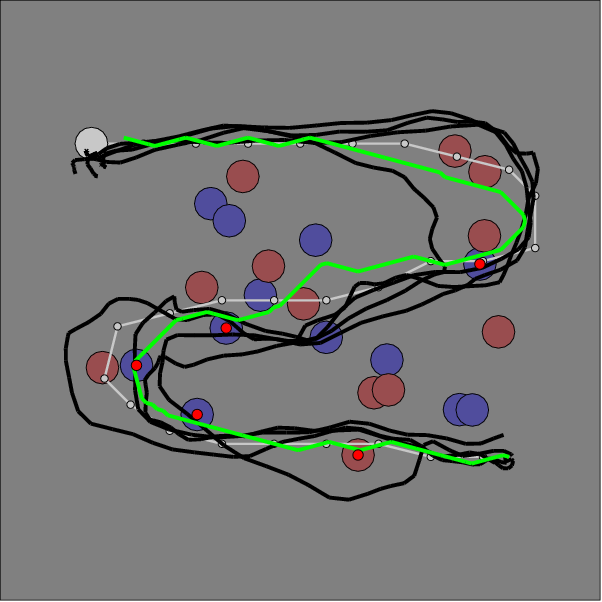
\includegraphics[width=\textwidth]{task_2.png}
\caption{Obstacle + Path,\\$w = (0.081, 0.264, 0.654)$. }
\end{subfigure}
\begin{subfigure}[b]{0.4\textwidth}
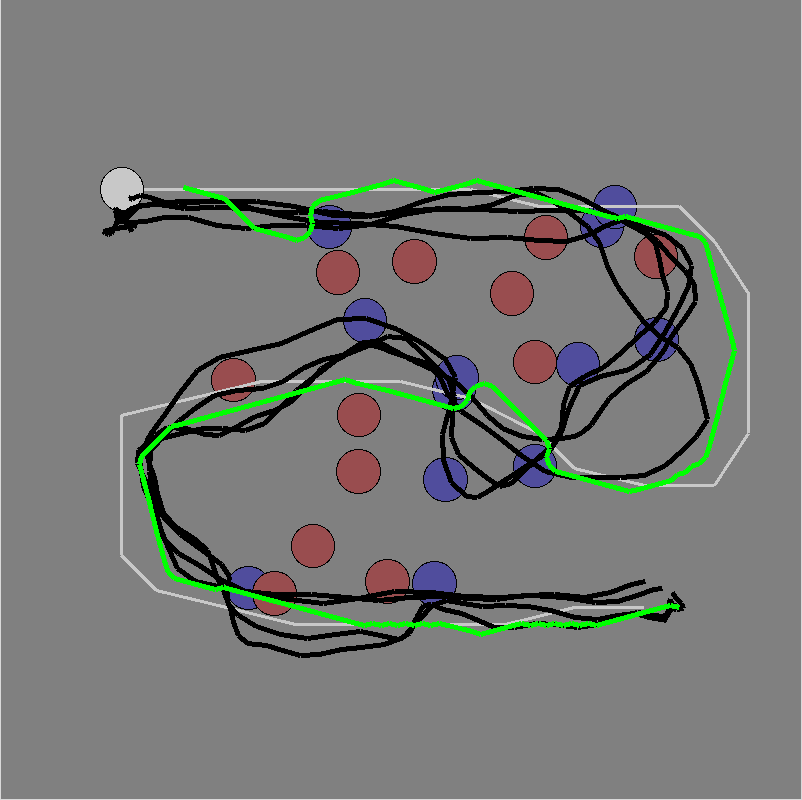
\includegraphics[width=\textwidth]{task_3.png}
\caption{Target + Path, \\$w = (0.254, 0.089, 0.655)$. }
\end{subfigure}
\begin{subfigure}[b]{0.4\textwidth}
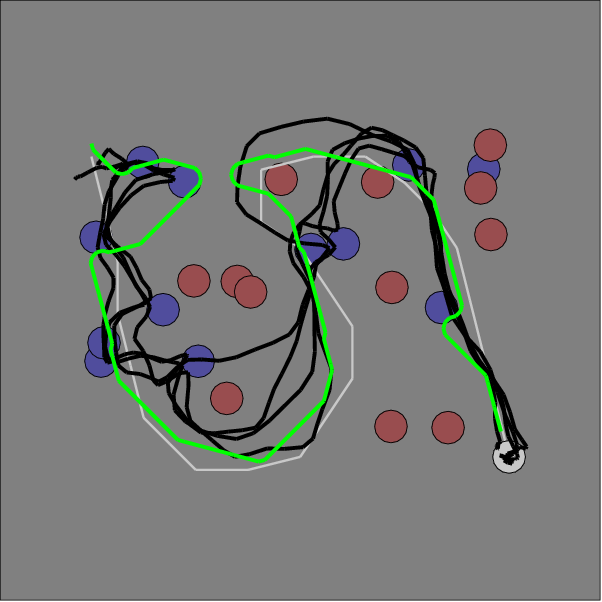
\includegraphics[width=\textwidth]{task_4.png}
\caption{Target + Obstacle + Path, \\$w = (0.215, 0.414, 0.369)$. }
\end{subfigure}
\caption{The trajectories of humans and the agent in the four tasks. Targets are blue and obstacles are red. The
black lines are trajectories of human subjects, and the green lines are
trajectories of the learning agent by using the optimum weights, $w$, derived
from modular inverse reinforcement learning. Weights for each task are given as (target,
obstacle, path).}
\label{fig:exp}
\end{figure}

\end{block}
\end{textblock}

% right
\begin{textblock}{37}(79,8)
\begin{block}{Experiments}
\begin{figure}[h]
\centering
\begin{subfigure}[b]{0.24\textwidth}
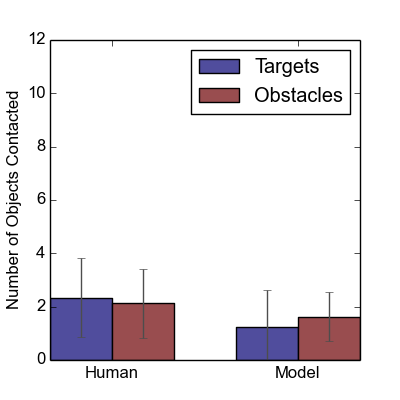
\includegraphics[width=\textwidth]{contact1.png}
\caption{Path module only.}
\end{subfigure}
\begin{subfigure}[b]{0.24\textwidth}
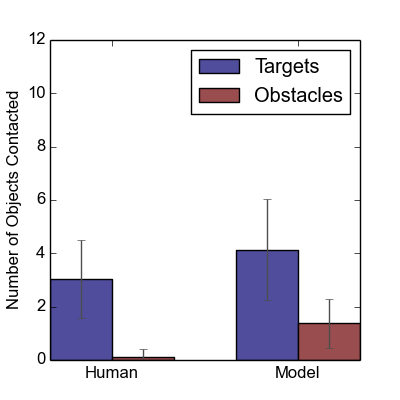
\includegraphics[width=\textwidth]{contact2.png}
\caption{Obstacle + Path.}
\end{subfigure}
\begin{subfigure}[b]{0.24\textwidth}
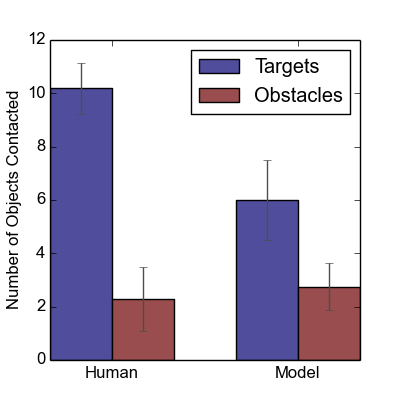
\includegraphics[width=\textwidth]{contact3.png}
\caption{Target + Path.}
\end{subfigure}
\begin{subfigure}[b]{0.24\textwidth}
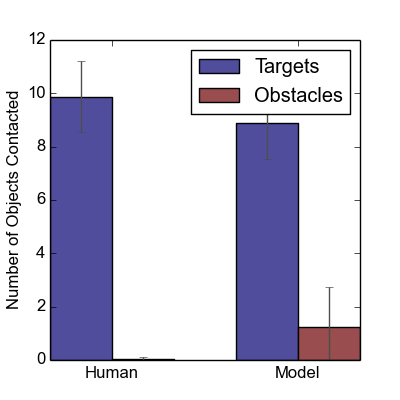
\includegraphics[width=\textwidth]{contact4.png}
\caption{All modules.}
\end{subfigure}
\caption{Number of targets hit and number of obstacles hit of the human subjects 
and the agent.}
\label{fig:stats}
\end{figure}

\begin{figure}[h]
\centering
\begin{subfigure}[b]{0.24\textwidth}
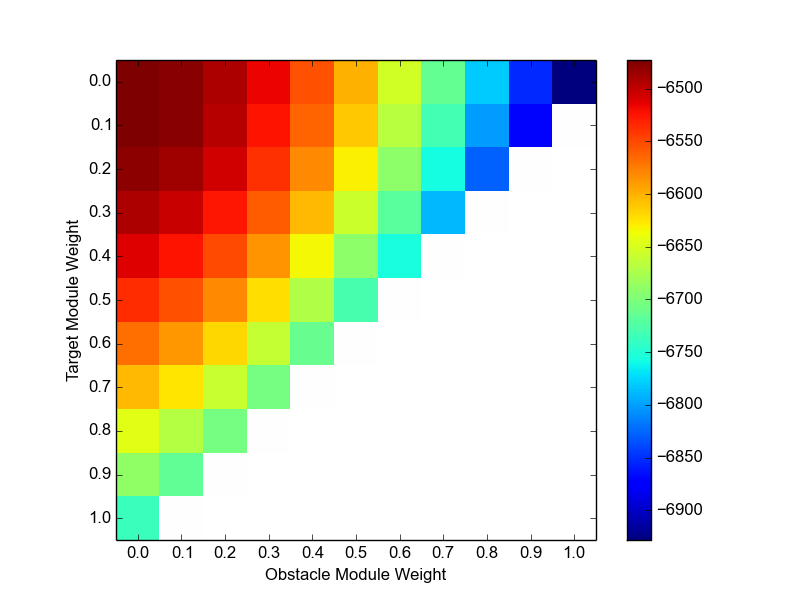
\includegraphics[width=\textwidth]{objValuesTask1.png}
\caption{Path following.}
\end{subfigure}
\begin{subfigure}[b]{0.24\textwidth}
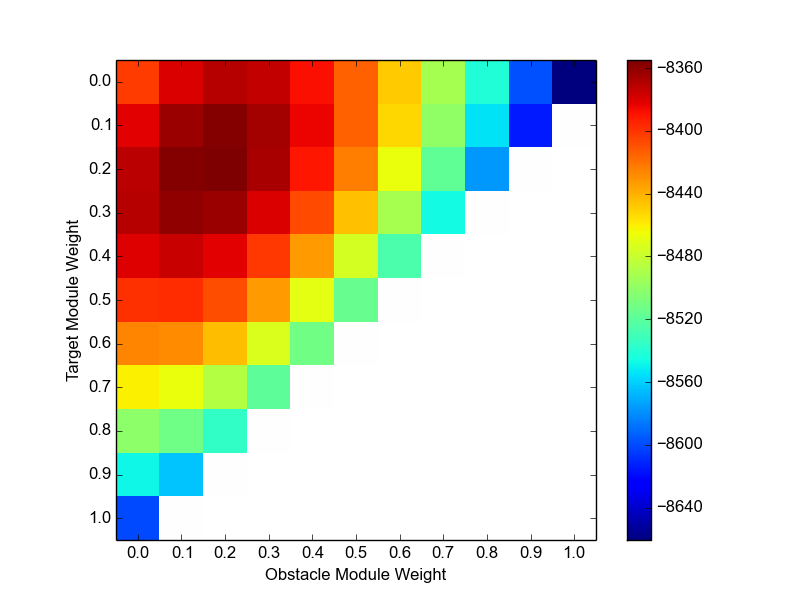
\includegraphics[width=\textwidth]{objValuesTask2.png}
\caption{Obstacle + Path. }
\end{subfigure}
\begin{subfigure}[b]{0.24\textwidth}
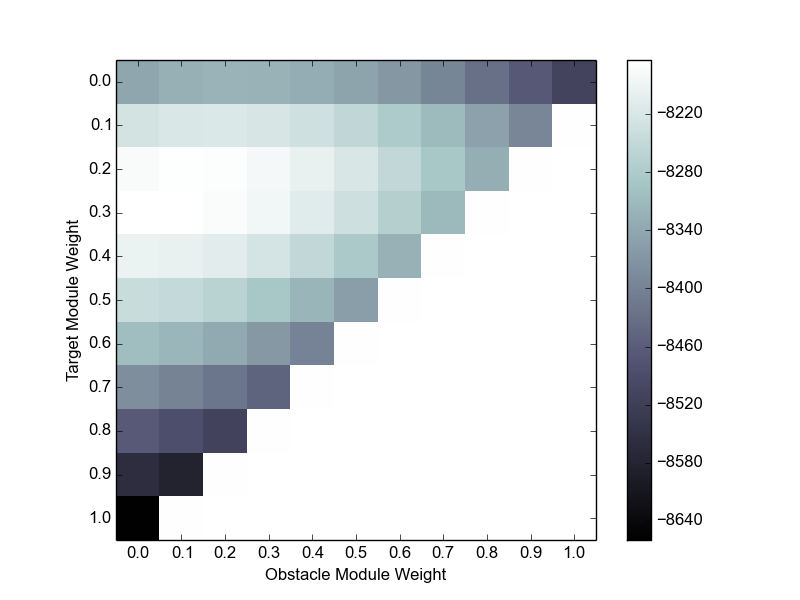
\includegraphics[width=\textwidth]{objValuesTask3.png}
\caption{Target + Path. }
\end{subfigure}
\begin{subfigure}[b]{0.24\textwidth}
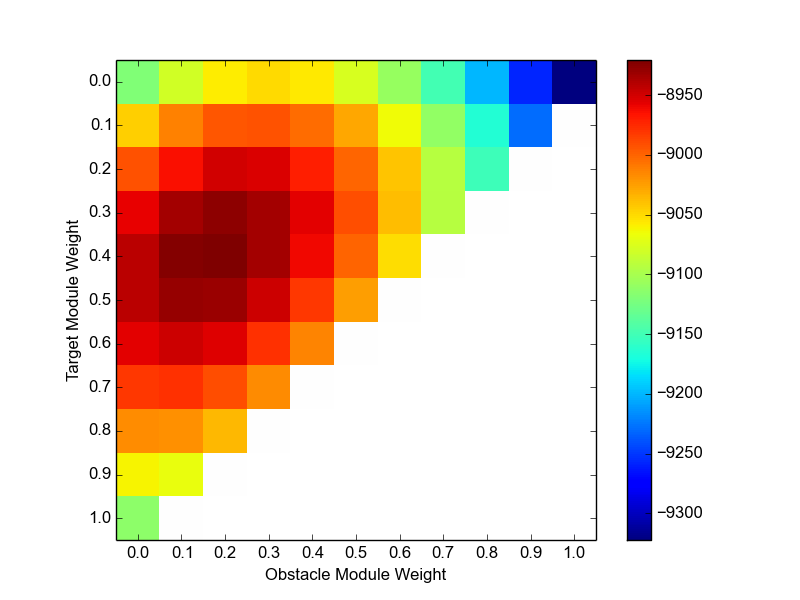
\includegraphics[width=\textwidth]{objValuesTask4.png}
\caption{All modules. }
\end{subfigure}
\caption{Heatmaps of the $\log$ of the likelihood for
different weights for the four tasks, respectively. The white zones indicate
higher probabilities. The weights of all three modules sum to 1, so we only show
the weights on the target and the obstacle modules.
}
\label{fig:heatmap}
\end{figure}
\end{block}

\begin{block}{Conclusion}
\begin{itemize}
\item
We analyzed human behavior using inverse modular reinforcement learning.
\item
The experimental results show that modular reinforcement learning can explain
human behavior well, even though the performance of the agent is currently
inferior to human subjects'.
\end{itemize}
\end{block}

\begin{block}{Following Work}
\begin{itemize}
\item
Learning weights (or rewards) and discounters of sub-MDPs simultaneously.
\item
Testing in gridworld domains, with hundreds of sub-MDPs. We compared Modular IRL
with Bayesian IRL in this condition.
\item
Evaluation by angular differences in policies, and likelihood of trajectories.
This is compared with other baseline agents.
\end{itemize}

{\bf Watch our follow-up paper in a future conference!}
\end{block}

\begin{block}{Acknowledgment}
\begin{itemize}
\item Funding.
\item Ruohan Zhang, on his separate work on modular reinforcement learning.
\end{itemize}
\end{block}

\end{textblock}

\end{frame}
\end{document}
